\section{The Platform}
\label{sec:platform}

The platform is a two-screen, researcher-operated system.
A participant reads reflowable Markdown-rendered text on a dedicated screen while a physical eye tracker streams gaze; on a second screen, a researcher console mirrors the participant's view live, overlays gaze, fixations, and saccade paths, and exposes the experiment controls.
Both surfaces are views of one authoritative, backend-owned session snapshot, so what the researcher sees is what the participant experiences (Figure~\ref{fig:ui}).

\begin{figure*}
  \centering
  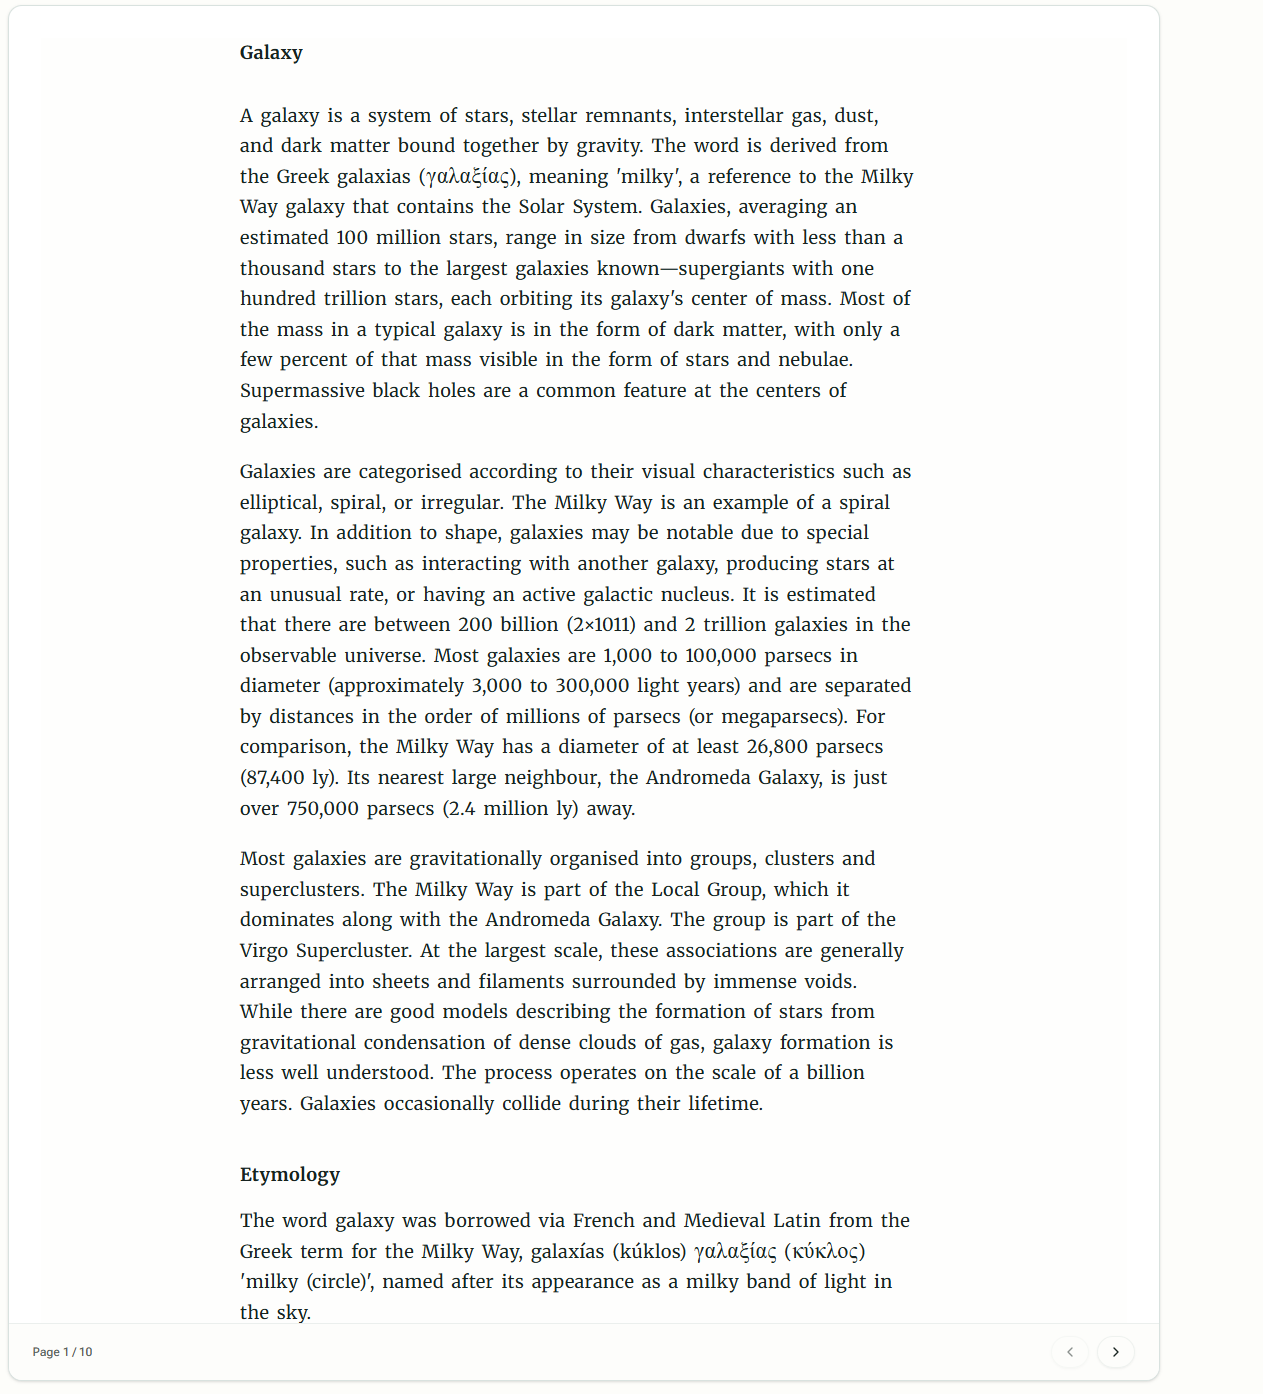
\includegraphics[height=62mm]{figures/ReadingView.png}\hspace{4mm}
  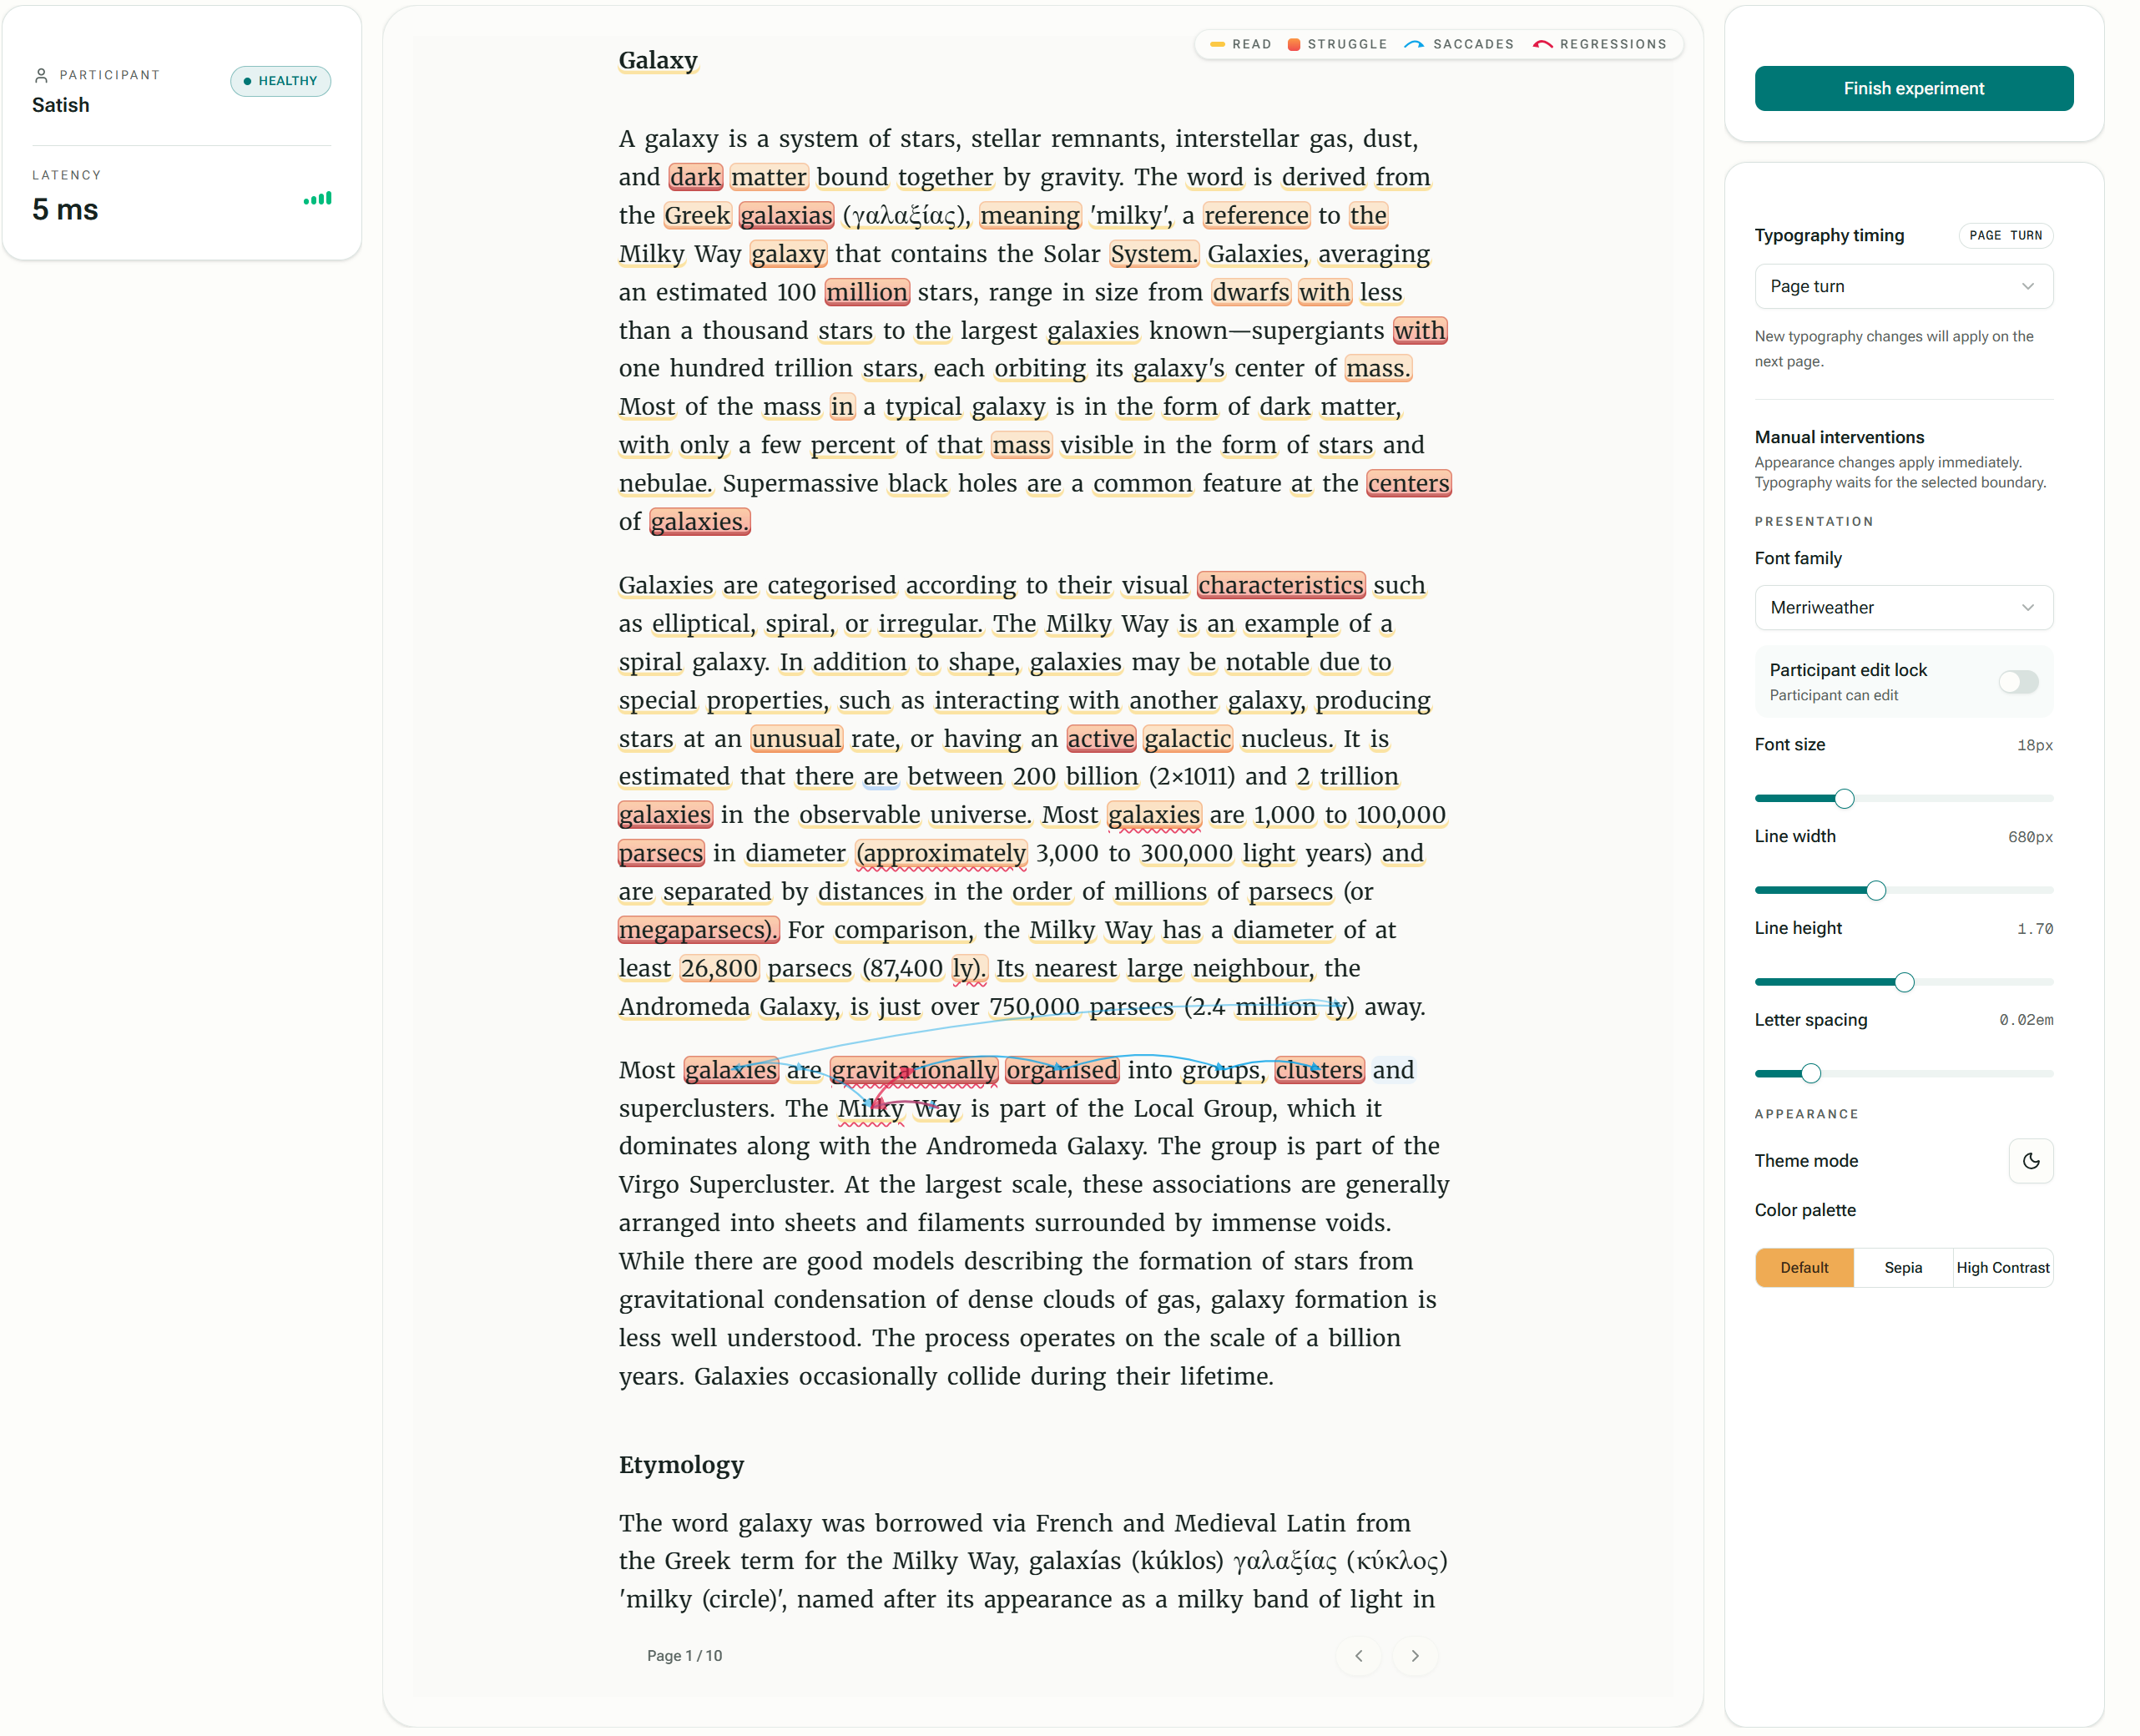
\includegraphics[height=62mm]{figures/ResearcherLiveView.png}
  \caption{The participant's reading view (left) and the researcher console mirroring the session live with gaze, fixation, and intervention controls (right).}
  \label{fig:ui}
\end{figure*}

\subsection{Four Modules Behind Stable Contracts}
\label{sec:modules}

The adaptive loop is decomposed into four modules, each independently replaceable behind a stable contract (Figure~\ref{fig:architecture}):

\begin{figure}
  \centering
  \begin{tikzpicture}[
    font=\footnotesize,
    mod/.style={draw, semithick, rounded corners=1.5pt, align=center,
      minimum height=6.5mm, text width=14.5mm, inner sep=1.5pt},
    seam/.style={align=center, text width=16mm, font=\scriptsize\itshape,
      inner sep=1pt},
    arr/.style={-{Stealth[length=2mm]}, semithick},
    node distance=4.5mm and 3.5mm]
    \node[mod] (sense) {Sensing};
    \node[mod, right=of sense] (ana) {Analysis};
    \node[mod, right=of ana] (dec) {Decision};
    \node[mod, right=of dec] (int) {Intervention};
    \draw[arr] (sense) -- (ana);
    \draw[arr] (ana) -- (dec);
    \draw[arr] (dec) -- (int);
    \node[seam, below=1.5mm of sense] {Tobii, webcam, simulated};
    \node[seam, below=1.5mm of ana] {built-in or external provider};
    \node[seam, below=1.5mm of dec] {manual, rules, or external};
    \node[seam, below=1.5mm of int] {typographic patch + restore};
    \node[draw, dashed, rounded corners=1.5pt, align=center,
      font=\scriptsize, above=4.5mm of dec, text width=17mm,
      inner sep=1.5pt] (res) {Researcher console};
    \draw[arr, dashed] (res) -- (dec);
    \draw[arr] (int.north) -- ++(0,12mm) -| (sense.north)
      node[pos=0.25, above, font=\scriptsize] {reflowed text, context preserved};
    \node[draw, rounded corners=1.5pt, align=center, font=\scriptsize,
      below=11mm of $(ana.south)!0.5!(dec.south)$, minimum width=68mm,
      inner sep=2pt]
      {every sample, event, decision, and intervention
       $\rightarrow$ replayable session record};
  \end{tikzpicture}
  \caption{The adaptive loop as four replaceable modules behind stable contracts; the researcher console gates decisions in advisory mode, and everything the loop produces lands in the replayable session record.}
  \label{fig:architecture}
\end{figure}

\begin{description}
\item[Sensing] produces gaze samples.
The default adapter wraps a Tobii eye tracker through the vendor SDK, including nine-point calibration gated on a validation pass; a simulated source implements the same contract for development and demonstration without hardware.
\item[Analysis] projects gaze into oculomotor events: fixations, saccades, and regressions.
A built-in dwell-based detector classifies fixations over text tokens in the spirit of area-of-interest identification~\cite{salvucci2000identifying}; alternatively, an external provider receives the gaze and reading observations and returns its own analysis.
\item[Decision] consumes the analysed state and returns at most one intervention proposal.
Strategies range from a built-in rule-based policy through researcher manual action to external providers, including machine-learning pipelines.
\item[Intervention] validates and commits a typographic change: font family and size, line width and height, letter spacing, and colour theme, applied as presentation patches to the participant's reader.
\end{description}

The backend follows a ports-and-adapters architecture whose dependency rule points strictly inward to a framework-free domain core.
The rule is not a convention: it is enforced at build time and additionally checked by an executable boundary test that inspects the compiled dependency graph.
Everything technology-specific, the Tobii SDK binding, the WebSocket transport, persistence, lives in adapters at the edge.

\subsection{Two Channels and a Lock-Free Hot Path}

Researcher commands travel over REST; high-frequency data travels over a dedicated WebSocket channel.
This separation keeps the per-sample path free of request overheads and locks: gaze ingestion uses atomic operations only, while a single lifecycle gate serialises control-plane operations such as session start and stop.
The latency budget for the full loop, from gaze sample to intervention dispatch, is 100\,ms, and Section~\ref{sec:evaluation} reports the measured margins.

External module providers connect out of process over a documented protocol: a hello/welcome handshake declaring the module and its capabilities, heartbeats, and typed inbound/outbound envelopes.
If a provider disconnects, the platform degrades gracefully to its built-in implementation and records the transition in the session record.

\subsection{Mapping Gaze to Words in a Reflowable Text}

Adaptive typography changes the very layout that gaze must be mapped onto, so the mapping cannot rely on static stimulus coordinates.
The reader maintains live bounding boxes for every rendered word token and maps each gaze sample in two stages: line selection with hysteresis, then within-line word scoring.
The hysteresis biases the mapping toward the currently attended line to absorb vertical jitter; because the mapping is computed against the current boxes, it survives reflow by construction and is independent of screen resolution.
Dwell accumulated per token feeds the analysis module, and per-token attention renders live in the researcher console.

\subsection{Context-Preserving Interventions}
\label{sec:context-preservation}

A typographic change that reflows the text can throw a reader to a different position, and prior work shows recovery is a measurable cost~\cite{jensen2025context}.
The platform separates a decision from its commit: an intervention decided now is committed at a controlled boundary, and the reader's context is carried across it.
The runtime captures a position anchor every 120\,ms, preferring the currently gazed word, falling back to the first visible word, then to the enclosing paragraph.
At commit, a restore strategy repositions the view: appearance-only changes preserve the scroll offset, while layout-affecting changes re-anchor to the captured word.
Crucially, the mechanism grades its own outcome: after every intervention it measures the residual distance between the restored anchor and its target and writes a graded outcome, preserved, degraded, or failed, with the pixel residual into the session record.
This self-instrumentation is what later exposed a defect in our own restore strategy (Section~\ref{sec:eval-context}).

\subsection{Researcher Control and Reproducible Sessions}

The researcher chooses among four execution modes: manual (researcher-applied interventions only), advisory (proposals await researcher approval), autonomous (proposals apply automatically), and control (no interventions).
A guided setup flow gates session start on four readiness checks: participant, tracker, calibration, and reading material.
During a session, every gaze sample, oculomotor event, proposal, decision, intervention, and context-restore outcome is appended to a single schema-versioned session record, checkpointed incrementally and sealed at session end.
Records export as JSON or CSV and reconstruct fully in a replay mode with timed playback and scrubbing; every quantitative result in this paper was computed from exported records alone, not from live state.
